\documentclass{article}
\usepackage{amsmath,mathtools}
\usepackage[usenames,dvipsnames]{xcolor}
\usepackage[bitstream-charter]{mathdesign}
\usepackage{microtype}
%\usepackage[utf8]{inputenc}
\usepackage[T1]{fontenc}
%\usepackage{libertine}
\usepackage{graphicx}
\usepackage{siunitx}

\usepackage{comment}
\usepackage{nicefrac}
\usepackage{booktabs}
\usepackage{float}
\usepackage{tikz}

%\usepackage[sfdefault]{AlegreyaSans} %% Option 'black' gives heavier bold face
%% The 'sfdefault' option to make the base font sans serif
%\renewcommand*\oldstylenums[1]{{\AlegreyaSansOsF #1}}

\floatstyle{plaintop}
\restylefloat{table}
\usepackage[justification=justified,singlelinecheck=false]{caption}
% header
\usepackage[backend=biber,sorting=none,autocite = superscript,natbib=true]{biblatex} \addbibresource{books.bib}
\usepackage{fancyhdr}
\fancyhf{}
\rhead{13.01.2017}
\lhead{Nevroz Arslan, Justin König Gruppe 6}
\setlength{\headheight}{15pt}
\rfoot{\thepage }
\lfoot{Versuch 2: IR-Spektroskopie}
\pagestyle{fancy}
%\renewcommand{\thesection}{\arabic{section}}% Remove section references...
%\renewcommand{\thesubsection}{\arabic{subsection}}%... from subsections
%\usepackage[backend=biber,sorting=none]{biblatex} \addbibresource{books.bib}

\usepackage{url} \usepackage{csquotes}
\sisetup{inter-unit-product=\ensuremath{{}\cdot{}}}
\renewcommand{\arraystretch}{1.5}
\definecolor{skyblue1}{RGB}{135, 206, 250}
\definecolor{flame}{RGB}{226, 88, 34}
\definecolor{scarletred1}{RGB}{252, 40, 71}
\definecolor{cyanblau}{RGB}{0, 158, 224}
\definecolor{charcoal}{rgb}{0.21, 0.27, 0.31}

\begin{document}

\section{Ziel des Versuches}
Der Versuch befasst sich mit der Infrarotspektroskopie und den physikalischen Ursachen der Schwingungen der Materie.
Dazu sollen Spektren von Kohlenmonoxid aufgenommen werden.
\section {Theorie\supercite{fadini}}
\subsection{Molekülschwingungen}
Die Wechselwirkung zwischen elektromagnetischer Strahlung und Molekülen
bildet die Grundlage verschiedener Methoden der Strukturbestimmung. Zu den wichtigsten
gehören diejenigen, die auf die Absorption der Strahlung (Infrarot Spektroskopie),
ihre Streuung (Raman Spektroskopie) oder Beugung (röntgenographische Methoden)
zurückzuführen sind.
Die Schwingungen treten im allgemein im mittleren IR-Bereich,
also bei Wellenzahlen 4000 \si{\per\centi\meter} und 200 \si{\per\centi\meter}.

In einem makroskopischen Modell stellt man ein zweiatomiges Molekül
durch zwei Massen m$_1$ und $_2$ dar, die durch eine elastische Feder verbunden sind.
Wenn der Gleichgewichtsabstand r$_e$ zwischen den beiden Massen um den Betrag $\delta r$
verzerrt und das System darauf losgelassen wird, so führt es eine Schwingungsbewegung
um die Gleichgewichtslage aus, die durch die rücktreibende Kraft $K$ verursacht wird. $K$
ist in erster Näherung zur Auslenkung proportional, jedoch entgegengerichtet:
\begin{equation}\label{eq:harmonisch}
K = - f \cdot \Delta r = -f \cdot (r_{max} -r_e)
\end{equation}
Der Proportionalitätsfaktor f, dem im Modell die Federkonstante entspricht,
wird bei der Beschreibung von Molekülschwingungen als Kraftkonstante bezeichnet.
Anschaulich ist $f$ ein Maß für die Bindungsstärke, deren Berechnung eine der wichtigsten
theoretischen Anwendungen der Schwingungsspektroskopie darstellt.
\begin{figure}
\centering
\resizebox {.6\linewidth} {!} {
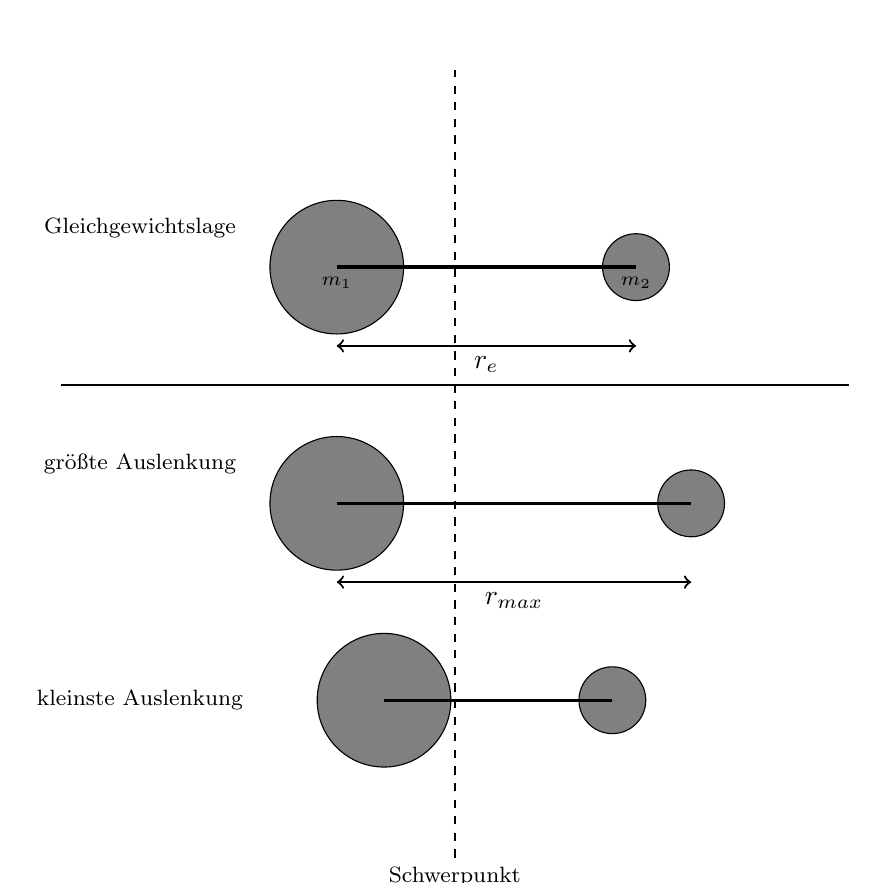
\begin{tikzpicture}

\node at (1,8) {\footnotesize Gleichgewichtslage};
\node at (1,5) {\footnotesize größte Auslenkung};
\node at (1,2) {\footnotesize kleinste Auslenkung};
\node at (5,-0.25) {\footnotesize Schwerpunkt};


\node[circle,fill=gray,draw=black,inner sep=6mm] at (4.1,2.0) (p1) {};
\node[circle,fill=gray,draw=black,inner sep=3mm] at (7,2.0) (p2) {};
\draw[very thick] (4.1,2.0) -- (7,2.0);



\node[circle,fill=gray,draw=black,inner sep=6mm] at (3.5,4.5) (p3) {};
\node[circle,fill=gray,draw=black,inner sep=3mm] at (8,4.5) (p4) {};
\draw[very thick] (3.5,4.5) -- (8,4.5) ;
\draw[<->,thick] (3.5,3.5) -- (8,3.5) node[midway,below] {$r_{max}$};


\draw[ thick]  (0,6) -- (10, 6) ;
\node[circle,fill=gray,draw=black,inner sep=6mm] at (3.5,7.5) (p5) {};
\node[circle,fill=gray,draw=black,inner sep=3mm] at (7.3,7.5) (p6) {};
\node (v1) at (3.5,7.3) {\scriptsize $m_1$};
\node (v2) at (7.3,7.3) {\scriptsize $m_2$};
\draw[<-> ,thick]  (3.5,6.5) -- (7.3,6.5)  node[midway,below] {$r_e$} ;


\draw[very thick] (3.5,7.5) -- (7.3,7.5);

\draw[ thick, dashed]  (5,0) -- (5,10) ;

\end{tikzpicture}
}
\caption{Das Modell eines schwingenden zweiatomigen Moleküls} \label{fig:M1}
\end{figure}

\subsubsection{Der harmonische Ansatz}
Die potentielle Energie als Funktion des Kernabstandes $r$ ergibt sich durch Integration zu
\begin{equation}
  v(r) = \frac{1}{2} \cdot (f \cdot (\Delta r)^2) = \frac{1}{2}(f \cdot (r -r_e)^2)
\end{equation}
und hat damit einen parabelförmigen Verlauf. Das Potential $V$ und die dadurch beschriebene Schwingungsbewegung werden,
da sie auf dem linearen Kraftgesetz beruhen~\ref{eq:harmonisch}, als \textit{harmonisch} bezeichnet.
Aus der quantentheoretischen Beschreibung des \glqq harmonischen Oszillators \grqq erhält man seine Energie-Eigenwerte $E _v$:
\begin{equation}
  E _v = h \cdot \nu ^{'}_{vib} \cdot (v +\frac{1}{2})
\end{equation}
Dabei ist $\nu ^{'}_{vib}$ die Frequenz der ausgeführten Schwingungsbewegung,
und die Schwingungsquantenzahl $v$ kennzeichnet Schwingungsniveaus,
so dass $v = 0$ dem Grundzustand mit der Energie $E _0 = \frac{1}{2} \cdot h \nu ^{'}_{vib} $ entspricht;
$v = 1$ bezeichnet den ersten angeregten Zustand ( $E _1 = \frac{3}{2} \cdot h \nu ^{'}_{vib} $) usw.
Der Abstand $\Delta E$ zwischen zwei benachbarten Schwingungsniveaus ist immer gleich ( $ \Delta E =  h \nu ^{'}_{vib} $ )
\begin{figure}[!ht]
  \centering
  \resizebox {.7\linewidth} {!} {
    \begin{tikzpicture}
      \def\xmin{0}
      \def\xmax{10}
      \def\ymin{0}
      \def\ymax{6}

      (\xmax,\ymax);
      \draw[->] (\xmin,\ymin) -- (\xmax,\ymin) node[right] {$r$};
      \draw[->] (\xmin,\ymin) -- (\xmin,\ymax) node[above] {$V(r)$};

      \node (v1) at (0.6,1.5) {\scriptsize $V = 0$};
      \node (v2) at (0.6,2.25) {\scriptsize $ V = 1$};
      \node (v3) at (0.6,3) {\scriptsize $ V = 2 $};
      \node (v4) at (0.6,3.75) {\scriptsize $ V = 3$};

      \node (e1) at (7.8,1.5) {\scriptsize $E_0 = \frac{1}{2} \cdot h \cdot v{'}$};
      \node (e2) at (7.8,2.25) {\scriptsize $E_1 = \frac{3}{2} \cdot h \cdot v{'}$};
      \node (e3) at (7.8,3) {\scriptsize $E_2 = \frac{5}{2} \cdot h \cdot v{'} $};
      \node (e4) at (7.8,3.75) {\scriptsize $ E_3 = \frac{7}{2} \cdot h \cdot v{'}$};

      \node (re) at (4, -0.25) {\scriptsize $ r _e$};

      \draw[] (3.12,1.5) -- (4.87,1.5);
      \draw[] (2.62,2.25) -- (5.37,2.25);
      \draw[] (2.25,3) -- (5.75,3);
      \draw[] (2,3.75) -- (6,3.75);

      \draw[<->, thick] (4,1.5) -- (4,2.25) ;
      \draw[<->, thick] (4,2.25) -- (4,3) ;
      \draw[<->, thick] (4,3) -- (4,3.75) ;

      \draw[ thick, dashed]  (1,1.5) -- (3.125,1.5) ;
      \draw[ thick, dashed]  (1,2.25) -- (2.5,2.25) ;
      \draw[ thick, dashed]  (1,3) -- (2.25,3) ;
      \draw[ thick, dashed]  (1,3.75) -- (1.75,3.75) ;

      \draw[ thick, dashed]  (5,1.5) -- (7,1.5) ;
      \draw[ thick, dashed]  (5.5,2.25) -- (7,2.25) ;
      \draw[ thick, dashed]  (5.75,3) -- (7,3) ;
      \draw[ thick, dashed]  (6.1,3.75) -- (7,3.75) ;

      \draw (1.25,6) parabola[parabola height=-5cm,thick] (6.75,6);
    \end{tikzpicture}
  }
  \caption{Potenialverlauf für den harmonischen Oszillator} \label{fig:M2}
\end{figure}


\subsubsection{Der anharmonische Ansatz}
Einige Phänomene wie die Dissoziation des Moleküls bei Zufuhr
hinreichend hoher Energie oder das Auftreten von Kombinations- und Oberschwingungen lassen sich durch den
harmonischen Ansatz nicht erklären. Eine realistischere Betrachtung ist mit einem erweiterterten Modell, dem des
\textit{anharmonischen Oszilattors}, möglich, dessen potentielle Energie annähernd durch das sog. Morse-Potential
beschrieben wird:
\begin{equation}
  V(r) = D \cdot [ 1- e^{-a(r-r_e)} ]^2
\end{equation}
Dies entspricht einer asymmetrischen Potentialkurve, deren Krümmung durch die Konstante $a$ charakterisiert wird. Der Faktor $D$
bedeutet die Summe aus Nullpunktsenergie $E _0$ und Dissoziationsenergie $E _D$.
\begin{figure}[!ht]
  \centering
  \resizebox {.7\linewidth} {!} {
    \begin{tikzpicture}
      \def\xmin{0}
      \def\xmax{10}
      \def\ymin{0}
      \def\ymax{6}

      (\xmax,\ymax);
      \draw[->] (\xmin,\ymin) -- (\xmax,\ymin) node[right] {$r$};
      \draw[->] (\xmin,\ymin) -- (\xmin,\ymax) node[above] {$V(r)$};

      \draw[] (1.25,6) parabola[parabola height=-4cm,very thick] bend (4.5,2) (6,3);
      \draw[] (6,3) .. controls (7,4.5) .. (10,4.5);

      \node (v0) at (0.6,1) {\scriptsize $V = 0$};
      \node (v1) at (0.6,2.25) {\scriptsize $ V = 1$};
      \node (v2) at (0.6,3) {\scriptsize $ V = 2 $};
      \node (v3) at (0.6,3.6) {\scriptsize $ V = 3$};

      \draw[ thick, dashed]  (1,1) -- (3.125,1) ;
      \draw[ thick, dashed]  (1,2.25) -- (2.5,2.25) ;
      \draw[ thick, dashed]  (1,3) -- (2.25,3) ;
      \draw[ thick, dashed]  (1,3.6) -- (1.75,3.6) ;

      \draw[ thick, dashed]  (4.75,1) -- (9,1) ;
      \draw[ thick, dashed]  (3.75,0.5) -- (10,0.5) ;

      \draw[thick, dashed]  (3.75,0) -- (3.75,0.5) ;
      \node (e0) at (8, 0.75) {\scriptsize $ E _0$};
      \draw[->,thick]  (8,0) -- (8,0.5) ;

      \draw[<-,thick]  (8,1) -- (8,2.25) ;
      \node (ed) at (8, 2.5) {\scriptsize $ E _D$};
      \draw[->,thick]  (8,2.75) -- (8,4.5) ;


      \draw[<-,thick]  (8.5,0.5) -- (8.5,2.3) ;
      \node (d) at (8.5, 2.5) {\scriptsize $ D$};
      \draw[->,thick]  (8.5,2.75) -- (8.5,4.5) ;


      \node (re) at (3.75, -0.25) {\scriptsize $ r _e$};

      \draw[] (2.9,1) -- (4.625,1);
      \draw[] (2.4,2.25) -- (5.45,2.25);
      \draw[] (2,3) -- (6,3);
      \draw[] (1.85,3.6) -- (6.4,3.6);

      \draw[->, thick] (3,1) -- (3,2.25) ;
      \draw[->, thick] (3.5,1) -- (3.5,3) ;
      \draw[->, thick] (4,1) -- (4,3.6) ;


    \end{tikzpicture}
  }
  \caption{Potenialverlauf für den anharmonischen Oszillator} \label{fig:M3}
\end{figure}

\subsection{IR-Spektroskopie}
Die Anregung einer \textit{Grundschwingung} kann dadurch beschrieben werden,
dass das Molekül unter Absorption eines Lichtquants vom 
Schwingungsgrundzustand in den nächsthöheren übergeht.
Dieser Vorgang ist nur dann möglich, 
wenn die damit verbundene Energieänderung 
gleich der Energie der einfallenden Lichtquanten ist:
\begin{equation}
  E _1 - E_0 = h. \nu ^{'}_{vib} = E _{LQ} = h \cdot \nu ^{'}_{LQ}
\end{equation}
Grundbedingung ist also, dass $\nu ^{'}_{vib} = \nu ^{'}_{LQ} $ ist ($LQ =$ Lichtquant). \par
Zur Aufnahme des Infrarot-Spektrums wird der Probe daher \textit{polychromatischer Strahlung} ausgesetzt,
deren Energie im mittleren IR-Bereich (3 \si{\nano\meter} - 50 \si{\nano\meter}) liegt; durch sukzessiven
Intensitätsvergleich mit einem die Probe nicht durchlaufenden Referenzstrahl können dann die Frequenzwerte
der absorbierten Strahlung festgestellt und somit die Schwingungsfrequenzen $\nu ^{'}_{vib} $ als Absolutwerte
ermittelt werden. \par
Als Folge der Anharmonizität sind neben dem Übergang eines Moleküls zum nächsthöheren Schwingungsniveau
(entsprechend der Auswahlregel $ \Delta v = +1$) auch solche mit $ \Delta v = +2, +3$ usw. erlaubt;
ihre Wahrscheinlichkeit und damit die Intensität der betreffenden Absorptionsbande nehmen
jedoch mit zunehmender Größe des Quantensprungs ab. Der Übergang $v =0 \rightarrow v =1$ entspricht der Grundschwingung,
$ v =0 \rightarrow v=2 $ der ersten Oberschwingung, die bei einer etwas kleineren als der doppelten Grundfrequenz
zu einer wesentlich schwächeren Bande führt, usw.
\subsection{Rotationsspektrum zweiatomiger Moleküle~\supercite{rovib}}
Das Modell zur Beschreibung von Rotationsübergängen 
ist das starre zweiatomige Molekül, auch als starrer Rotator bezeichnet. 
Beim starren Rotator sind zwei Atome mit den Massen $m_1$ und $m_2$ 
durch eine starre Bindung mit der Länge $r_0$ verbunden. 
Die Energie der Rotation ist quantisiert und erhält man nach Lösen 
der entsprechenden Schrödinger-Gleichung folgende Energieeigenwerte der Rotation:
\begin{equation}
\label{eq:erot}
E_{rot} = hc B J (J+1) \,\, \text{ mit } J = 0, 1,2 
\end{equation}

\begin{equation}
\label{eq:bconst}
B = \frac{h}{8 \ pi ^2 c I} ; (B in cm^{-1})  
\end{equation}
wobei $I$ das Trägheitsmoment des Moleküls, 
wie folgt zu berechnen ist.
\begin{align}
\label{eq:trag}
I &=\frac{m_1 m_2 }{m_1 + m_2} r_0^2\\
&=\mu r_0^2
\end{align}
Der Ausdruck $\mu$ ist die reduzierte Masse.
$B$ wird als Rotationskonstante bezeichnet; aus ihr kann die Bindungslänge des Moleküls
$r_0$ bestimmt werden. Die Rotationsenergieniveaus sind nicht äquidistant, sie
wachsen quadratisch mit der Rotationsquantenzahl J an.

\subsection{Interferometer}

\section{Auswertung}

\subsection{Untersuchung der Spektren}

Bei der Aufnahme der Spektren wurden die Auflösung sowie die Scanzahl variiert. Anhand der aufgenommenen Spektren wird ersichtlich, das mit höhere Scanzahl und Auflösung die Spektren deutlicher sind als mit geringerer Auflösung und Scanzahl. 
Wird die Anzahl der Scans bei einer Messung erhöht, so wird das Rauschen geringer und die Peaks können deutlicher erkannt werden. Bei niedriger Auflösung verschwimmen die Peaks wobei man bei einer höher gewählten Auflösung die Peaks besser unterscheiden kann.

Im Hintergrundsspektrum lassen sich Peaks bei einer Wellenzahl von circa 3600 \si{\per\centi\meter} und 1595 \si{\per\centi\meter}  
erkennen, welche für Wasser sprechen. Die sind tatsächlich drei normalen Modi des Wasser-Moleküls \supercite{atkins}. 
\begin{table}[htpb]
  \caption{Schwingungsfrequenzen von $H_2O$ aus der Literatur~\supercite{atkins}}
  \label{tab:label}
  \begin{tabular}{llc}
    $v_1$ & 3652 \si{\per\centi\meter} & Streck\\  
    $v_2$ & 1595 \si{\per\centi\meter} & Deformations \\  
    $v_3$ & 3756 \si{\per\centi\meter} & Streck\\  
  \end{tabular}
\end{table}
sowie bei den Wellenzahlen von circa 2250-2400 \si{\per\centi\meter} erkennt man die Peaks von $CO_2$.
Anhand der Tabelle~\ref{tab:chsc} aus dem Literatur\supercite{atkins} (S. 462) lässt sich festsellen, dass es in der Probekammer $CH_4$ vorhanden sein.  
\begin{table}[htpb]
  \caption{Typische Kohlenstoff Schwingungen}
  \label{tab:chsc}
  \begin{tabular}{ccl}
    Schwingungsart & $\tilde{\nu}$ \si{\per\centi\meter} \\
    C-H stretch & 2850–2960 \\
C-H bend & 1340–1465 \\
C-C stretch& 700-1230 \\
C=C stretch & 1620–1680
  \end{tabular}

\end{table}
Am besten sollte bei hoher Auflösung und einer hohen Scanzahl messen, da die Spektren so am deutlichsten lesbar sind. 
Dies lässt sich durch einen Vergleich von Spektren am \textit{Anhang I} und am \textit{Anhang II} mit dem am \textit{Anhang III} verdeutlichen.

\subsection{Bestimmung der Bindungslänge des CO-Moleküls}
In dem Versuch sollte die Bindungslänge des CO-Moleküls mit Hilfe der 

Die Werte, die für die Kombinationsdifferenz benötigt werden sind im R- bzw. P-Zweig enthalten. 
Hierzu werden zunächste die Rotationskonstanten $B_0$ und $B_1$ benötigt.
Durch Auftragung von $\Delta \tilde {\nu}$ gegen $J+0.5$ wird eine Gerade erhalten, 
mit deren Steigung die Rotationskonstanten berechnet werden können. 
Für den Grundzustand ergeben sich somit folgende Werte:


\subsection{Bestimmung der Dissoziationsenergie des CO-Moleküls}

Die Dissoziationsenergie kann mit Hilfe der Birge-Spooner-Extrapolation berechnet werden. Hierfür werden zunächst die Werte des Q-Zweiges aus den Mittelwerten der ersten Übergänge des P- und R-Zweiges ermittelt.
Die verwendeten Werte für die Birge-Spooner-Extrapolation betragen somit:



%\printbibliography
\end{document}
